
\begin{figure}[htb]
  % Requires \usepackage{graphicx}
  \centering
  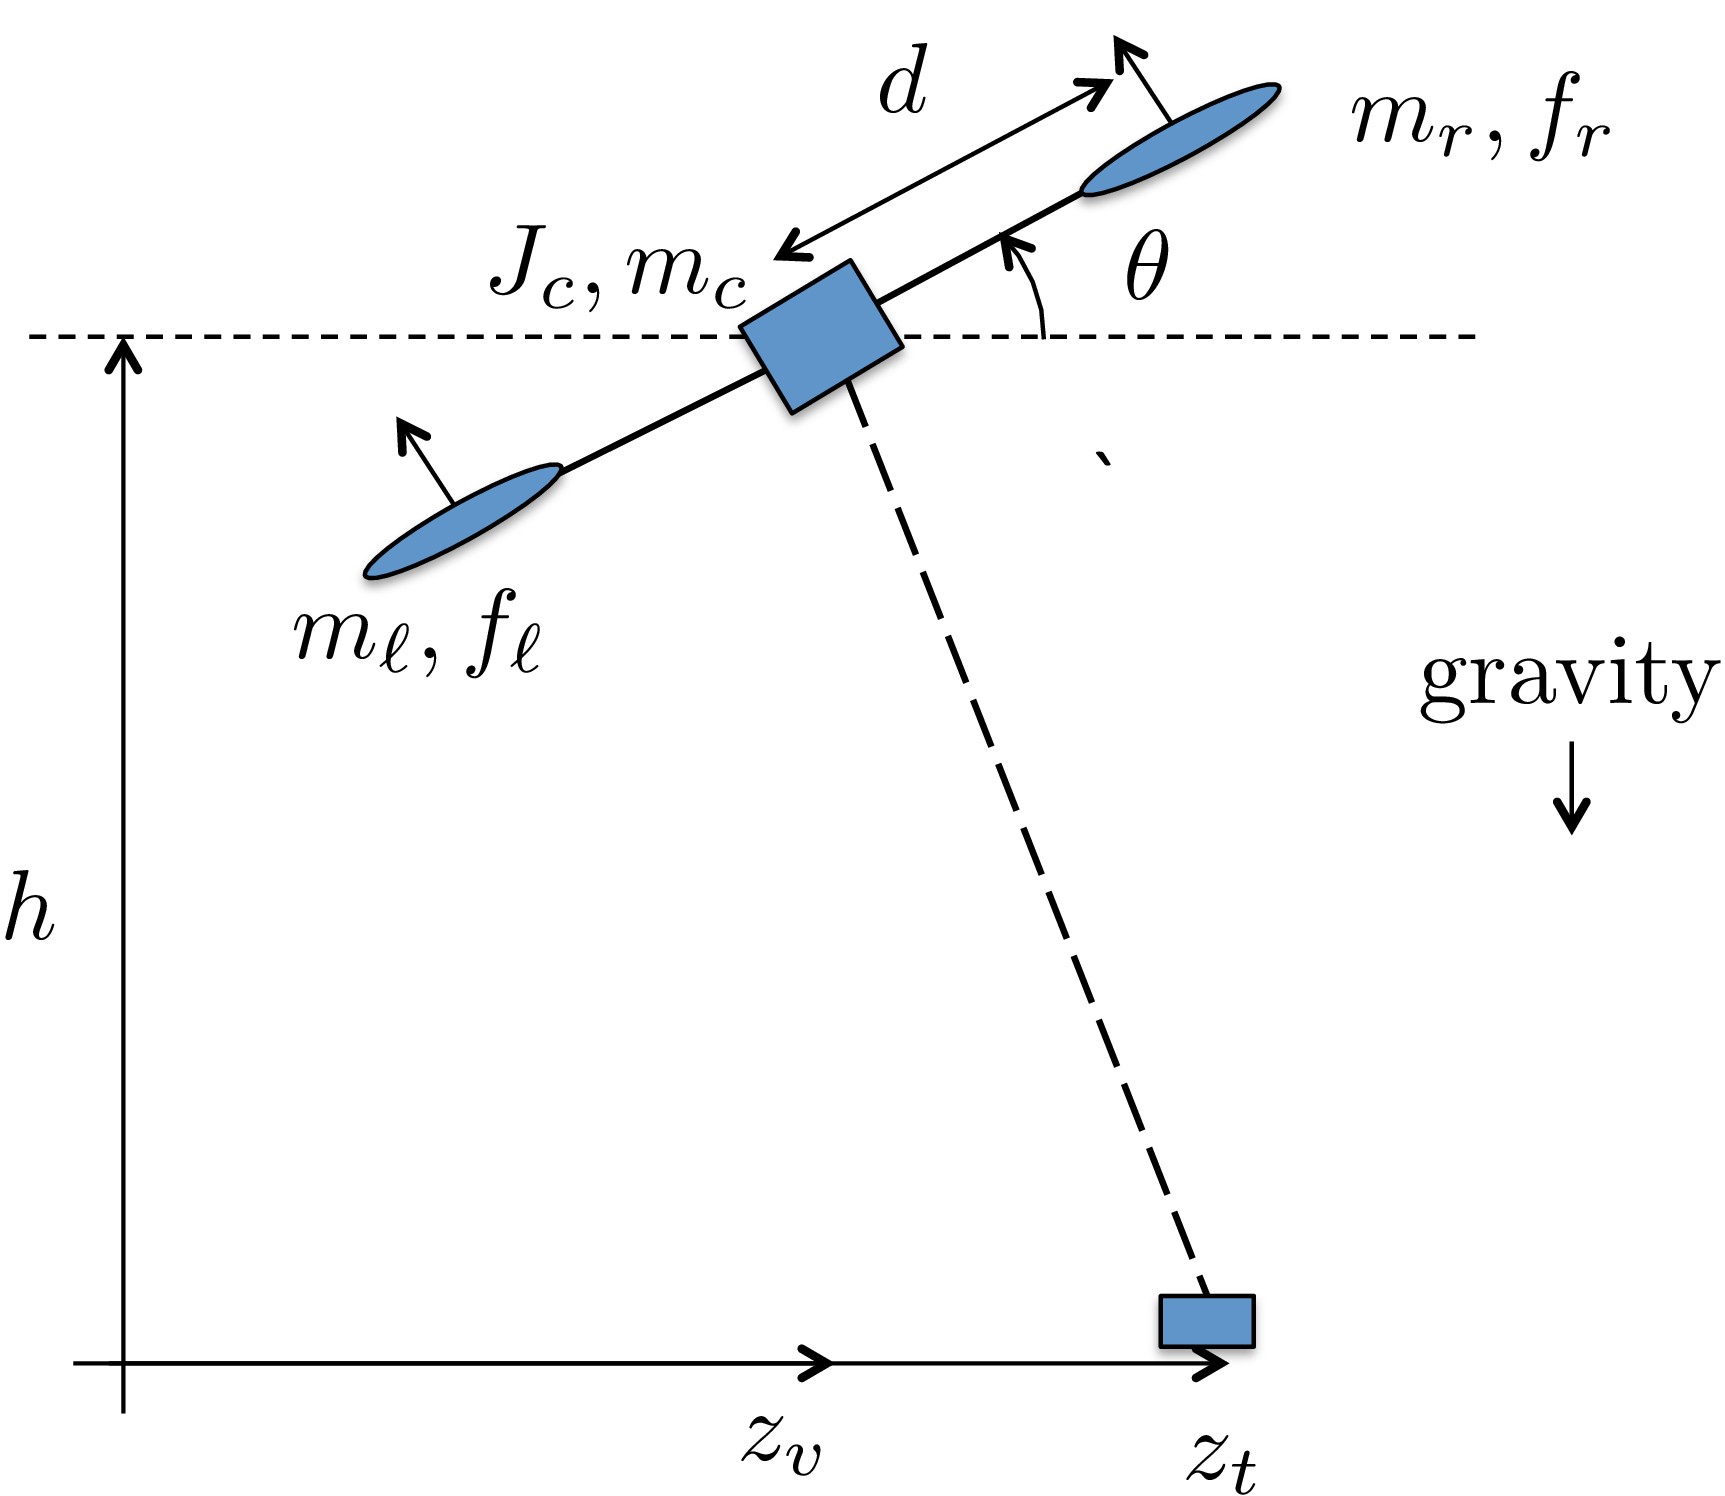
\includegraphics[width=0.8\textwidth]{6_design_studies/figures/hw_planar_VTOL_defn}
  \caption{Finding the equations of motion for the planar VTOL system.}
  \label{fig:hw_planar_VTOL_defn}
\end{figure}

The generalized coordinates for the system are the lateral position of the center pod $z$, the altitude of the center pod $h$, and the angle of the rotors $\theta$.  Therefore, let $\mathbf{q} = (z, h, \theta)^\top$.

Let $P_0$ be the potential energy when $z=0$, $h=0$, and $\theta=0$.  Then the potential energy of the planar VTOL system is the sum of the potential energy of the center of mass center pod, and the potential energy of each rotor, modeled as a point mass:
\begin{align*}
  P &= P_0 + m_c g h + m_r g (h + d \sin\theta) + m_l g (h - d \sin\theta)  \\
    &= (m_c + 2 m_r) g h + P_0.
\end{align*}

The external forces acting in the direction of $z$, $h$, and $\theta$ are
\begin{align*}
  \tau_1 &= -(f_r + f_l) \sin\theta \\
  \tau_2 &= (f_r + f_l) \cos\theta \\
  \tau_3 &= d (f_r - f_l).
\end{align*}
Momentum drag induces a viscous friction term in the direction of $z$, therefore
\[
-B\dot{\mathbf{q}} = \begin{pmatrix} -\mu & 0 & 0 \\ 0 & 0 & 0 \\ 0 & 0 & 0 \end{pmatrix}\begin{pmatrix} \dot{z} \\ \dot{h} \\ \dot{\theta} \end{pmatrix} = \begin{pmatrix} -\mu \dot{z} \\ 0 \\ 0 \end{pmatrix}.
\]

From problem \ref{hw:vtol}.1, the kinetic energy is
\begin{align*}
  K &= \frac{1}{2} (m_c + 2 m_r) \dot{z}^2 + \frac{1}{2} (m_c + 2 m_r) \dot{h}^2 + \frac{1}{2}\left(J_c + 2 m_r d^2 \right) \dot{\theta}^2.
\end{align*}
The Lagrangian is therefore given by
\[
L = \frac{1}{2} (m_c + 2 m_r) \dot{z}^2 + \frac{1}{2} (m_c + 2 m_r) \dot{h}^2 + \frac{1}{2}(J_c + 2 m_r d^2 ) \dot{\theta}^2 - (m_c + 2 m_r) g h - P_0.
\]
The Euler Lagrange equations are
\begin{align*}
\frac{d}{dt} \left( \frac{\partial L}{\partial \dot{z}} \right) - \frac{\partial L}{\partial z} &= \tau_1 - \mu\dot{z} \\
\frac{d}{dt} \left( \frac{\partial L}{\partial \dot{h}} \right) - \frac{\partial L}{\partial h} &= \tau_2 \\
\frac{d}{dt} \left( \frac{\partial L}{\partial \dot{\theta}} \right) - \frac{\partial L}{\partial \theta} &= \tau_3,
\end{align*}
where
\begin{align*}
\frac{\partial L}{\partial \dot{z}} &= (m_c + 2 m_r) \dot{z} \\
\frac{d}{dt} \left( \frac{\partial L}{\partial \dot{z}} \right) &= (m_c + 2 m_r) \ddot{z} \\
\frac{\partial L}{\partial z} &= 0 \\
\\
\frac{\partial L}{\partial \dot{h}} &= (m_c + 2 m_r) \dot{h} \\
\frac{d}{dt} \left( \frac{\partial L}{\partial \dot{h}} \right) &= (m_c + 2 m_r) \ddot{h} \\
\frac{\partial L}{\partial h} &= - (m_c + 2 m_r) g\\
\\
\frac{\partial L}{\partial \dot{\theta}} &= (J_c + 2 m_r d^2) \dot{\theta} \\
\frac{d}{dt} \left( \frac{\partial L}{\partial \dot{\theta}} \right) &= (J_c + 2 m_r d^2) \ddot{\theta} \\
\frac{\partial L}{\partial \theta} &= 0. \\
\end{align*}

Therefore the equations of motion are
\begin{align*}
(m_c + 2 m_r) \ddot{z} &= -(f_r + f_l) \sin\theta - \mu \dot{z} \\
(m_c + 2 m_r) \ddot{h}  + (m_c + 2 m_r) g &= (f_r + f_l) \cos\theta \\
\left( J_c + 2 m_r d^2 \right) \ddot{\theta} &= d \left( f_r - f_l \right)
\end{align*}

Using matrix notation, this equation can be rearranged to isolate the second order derivatives on the left and side
\begin{equation}\label{eq:vtol_sim_model}
\begin{pmatrix}
m_c + 2 m_r & 0           & 0 \\
0           & m_c + 2 m_r & 0 \\
0           & 0           & J_c + 2 m_r d^2
\end{pmatrix}
\begin{pmatrix}
\ddot{z} \\
\ddot{h} \\
\ddot{\theta}
\end{pmatrix}
=
\begin{pmatrix}
-(f_r + f_l) \sin\theta - \mu\dot{z} \\
-(m_c + 2 m_r) g + (f_r + f_l) \cos\theta \\
d \left( f_r - f_l \right)
\end{pmatrix}.
\end{equation}
Equation~\eqref{eq:vtol_sim_model} represents the simulation model for the ball on beam system.
